% Slides for 2025-08-05
% To create a slide, use the following:
% \begin{frame}{TITLE}
%     BODY
% \end{frame}

% To create a slide with a bullet list, use the following:
% \begin{frame}{TITLE}
%     \begin{itemize}
%         \item ITEM 1
%         \item ITEM 2
%     \end{itemize}    
% \end{frame}

% To create a slide with numbered list, use the following:
% \begin{frame}{TITLE}
%     \begin{enumerate}
%         \item ITEM 1
%         \item ITEM 2
%     \end{enumerate}
% \end{frame}

% To create a slide with a graphic:
% 1. Add the graphic to this folder (named picture.png)
% 2. Use the following:
% \begin{frame}{TITLE}
%     \centering
%     \includegraphics[height=0.7\textheight,width=0.7\textwidth,keepaspectratio]{picture.png}
% \end{frame}

% To create a slide with two columns, use the following:
% \begin{frame}{TITLE}
%     \begin{columns}
%         \begin{column}{0.5\textwidth}
%             COLUMN 1 BODY
%         \end{column}
%         \begin{column}{0.5\textwidth}
%             COLUMN 2 BODY
%         \end{column}
%     \end{columns}
% \end{frame}

\begin{frame}{ML Team Agenda}
    \begin{itemize}
        \item Desktop App
        \item Knowledge Graphs
        \item Regression
        \item Template Matching
        \item Binary Classifier
        \item Site Separation
        \item D3.JS Visualization
    \end{itemize}
\end{frame}

\begin{frame}{Desktop App}
    \begin{itemize}
        \item Sent to collaborators for feedback, scheduling meeting to address issues
    \end{itemize}
    \begin{figure}
        \centering
        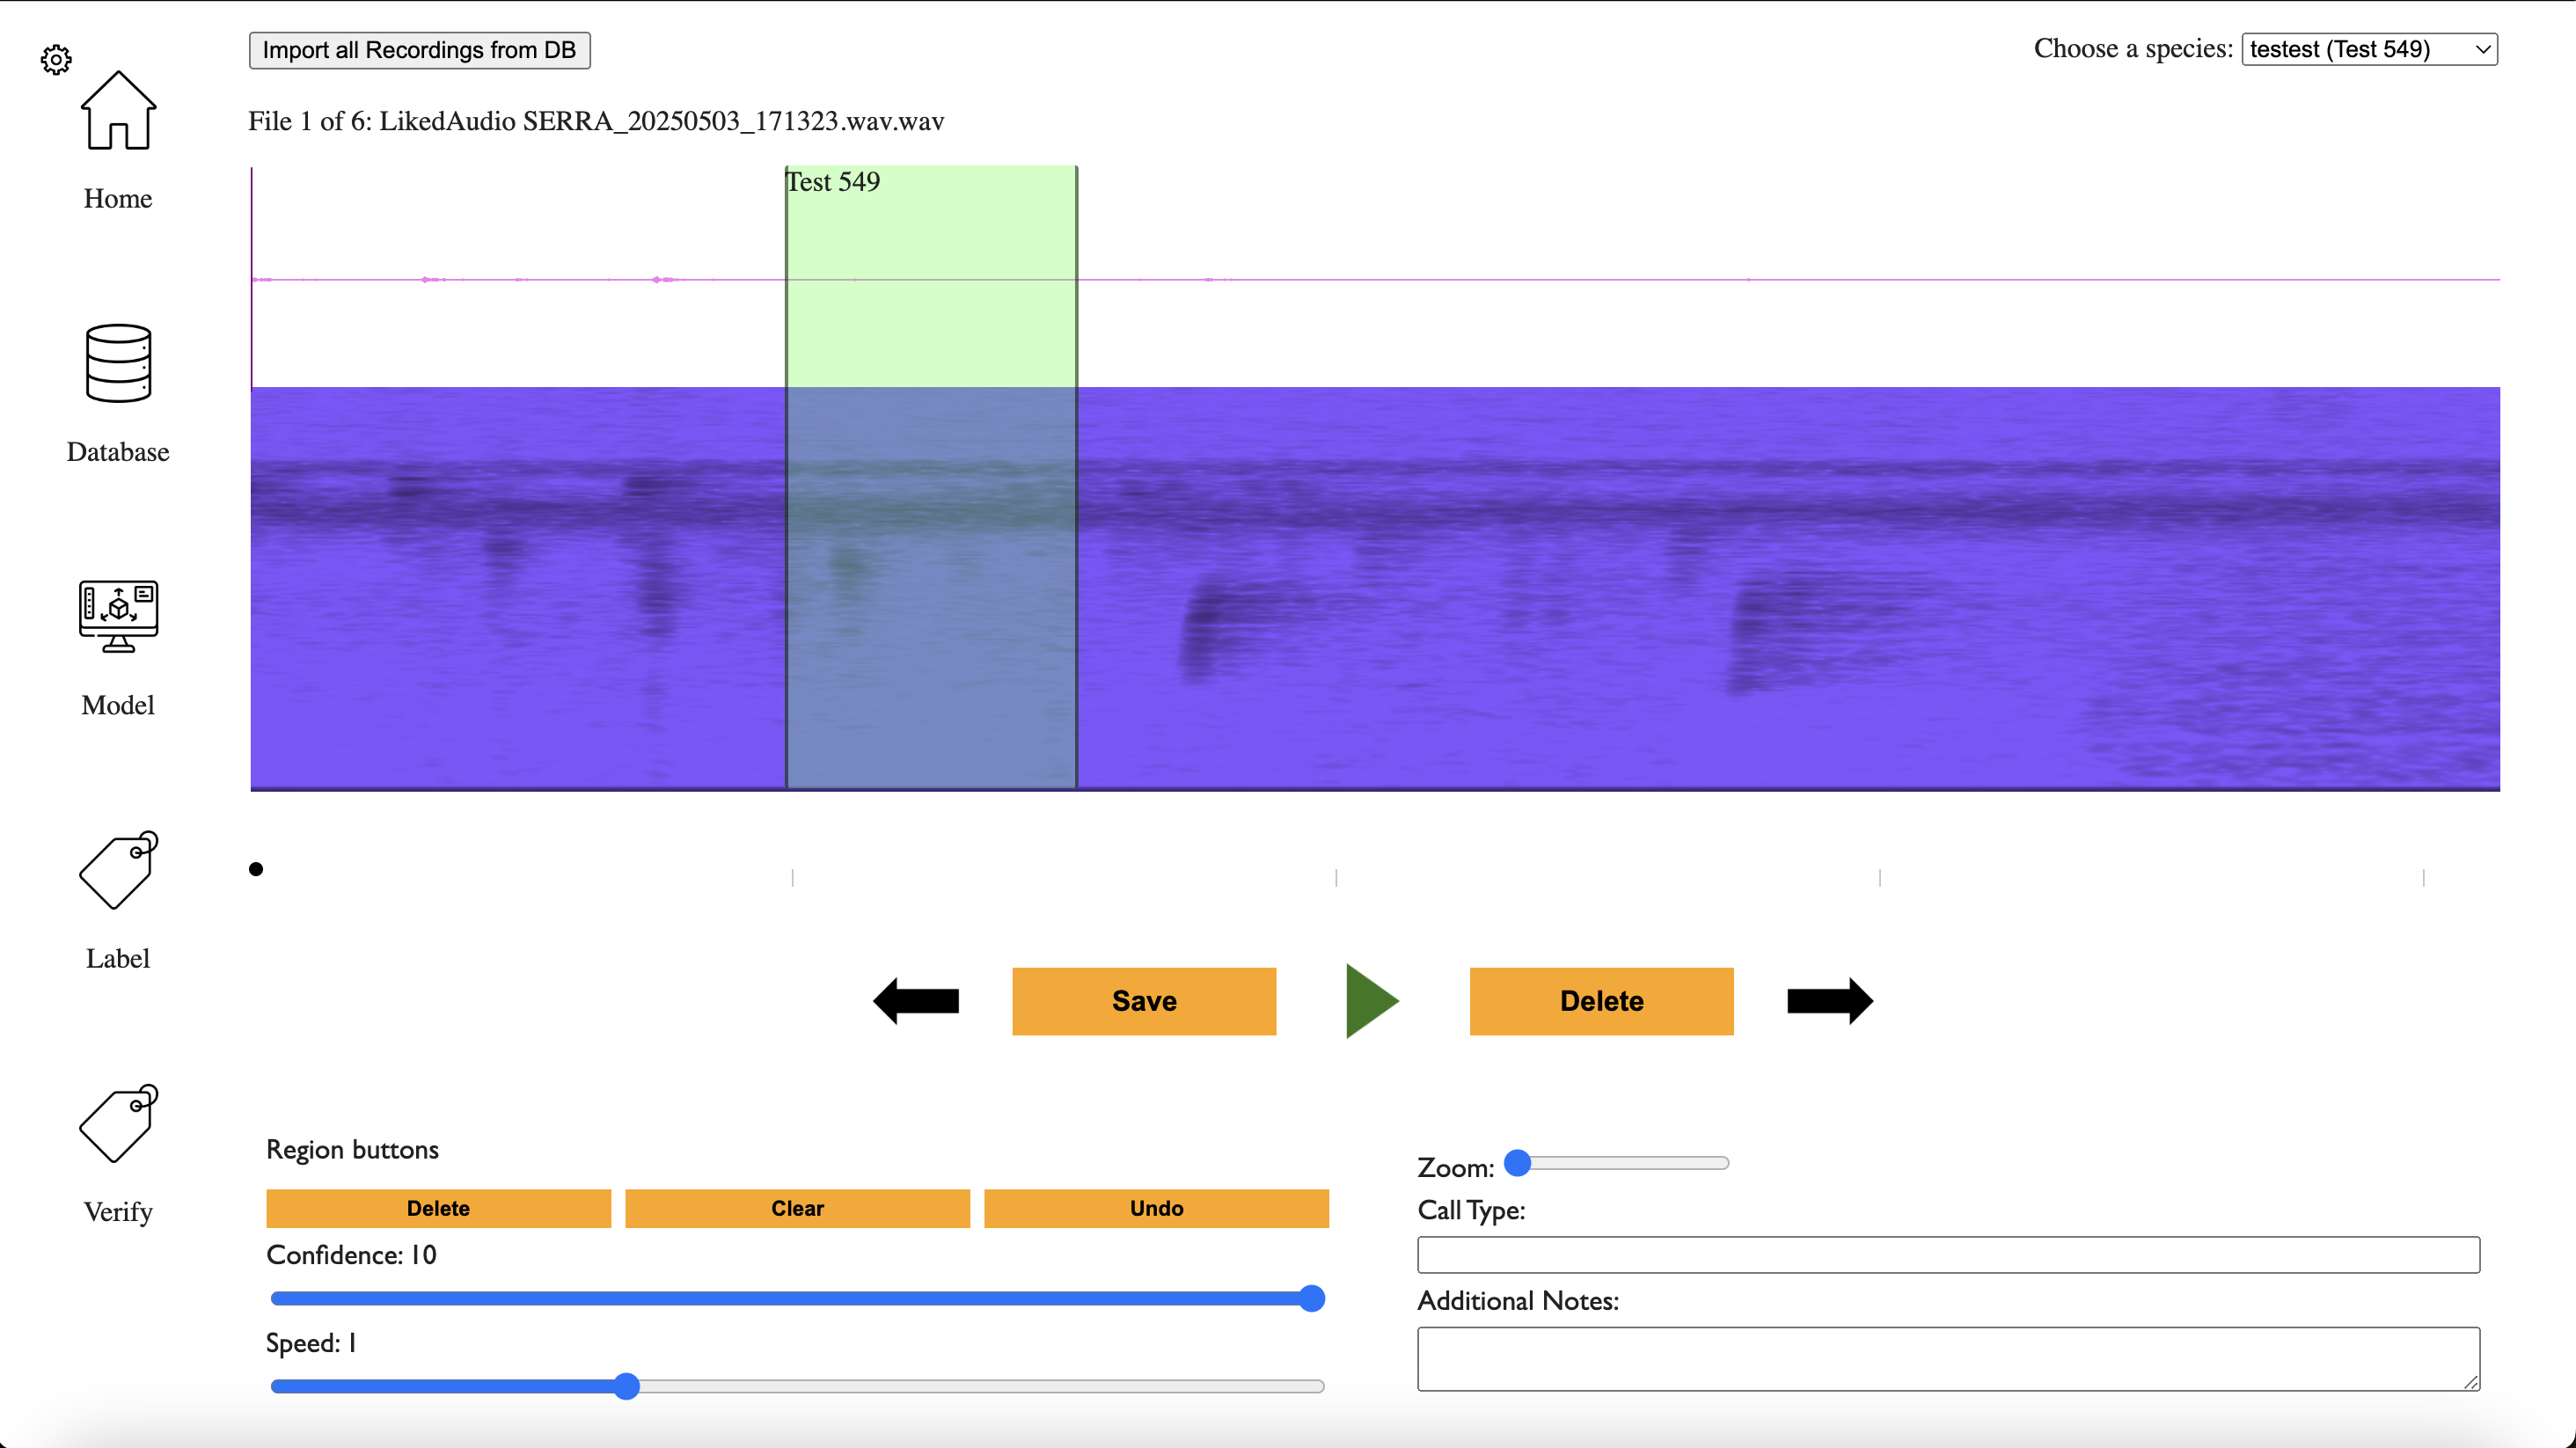
\includegraphics[height=0.7\textheight,width=0.7\textwidth,keepaspectratio]{images/desktop_app_1.png}
        \caption{Desktop App interface}
    \end{figure}
\end{frame}

\begin{frame}{Desktop App}
    \begin{figure}
        \centering
        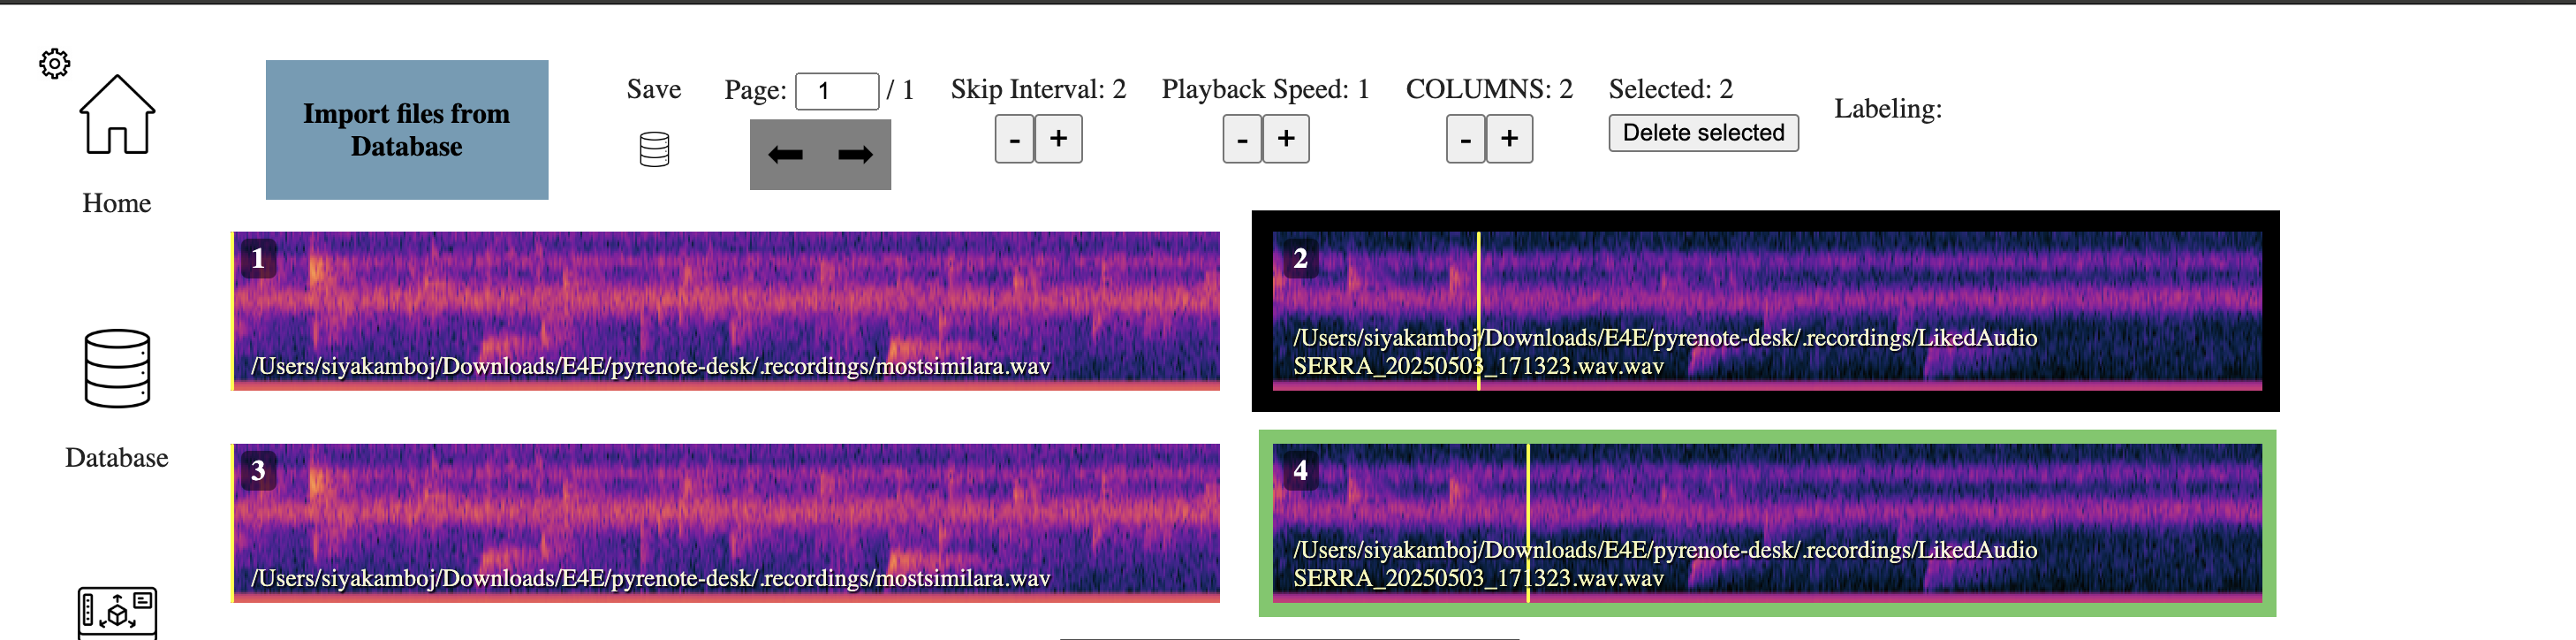
\includegraphics[height=1.0\textheight,width=1.0\textwidth,keepaspectratio]{images/desktop_app_2.png}
        \caption{Desktop App labeling interface}
    \end{figure}
\end{frame}

\begin{frame}{Knowledge Graphs - Input}
    \begin{columns}
        \begin{column}{0.3\textwidth}
            \begin{itemize}
                \item Inserted 2,231 of Paola's audio files
            \end{itemize}
        \end{column}
        \begin{column}{0.7\textwidth}
            \centering
            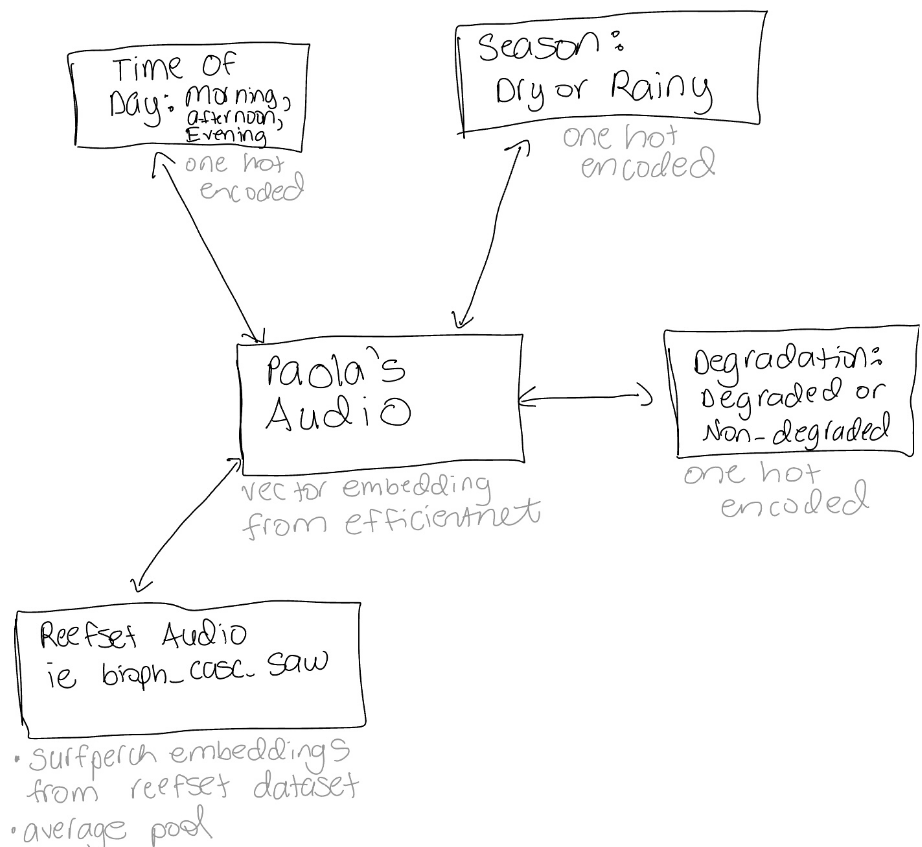
\includegraphics[height=0.8\textheight,width=0.8\textwidth,keepaspectratio]{images/knowledge_graph.png}
        \end{column}
    \end{columns}
\end{frame}

\begin{frame}{Knowledge Graphs - Results}
    \begin{columns}
        \begin{column}{0.7\textwidth}
            \centering
            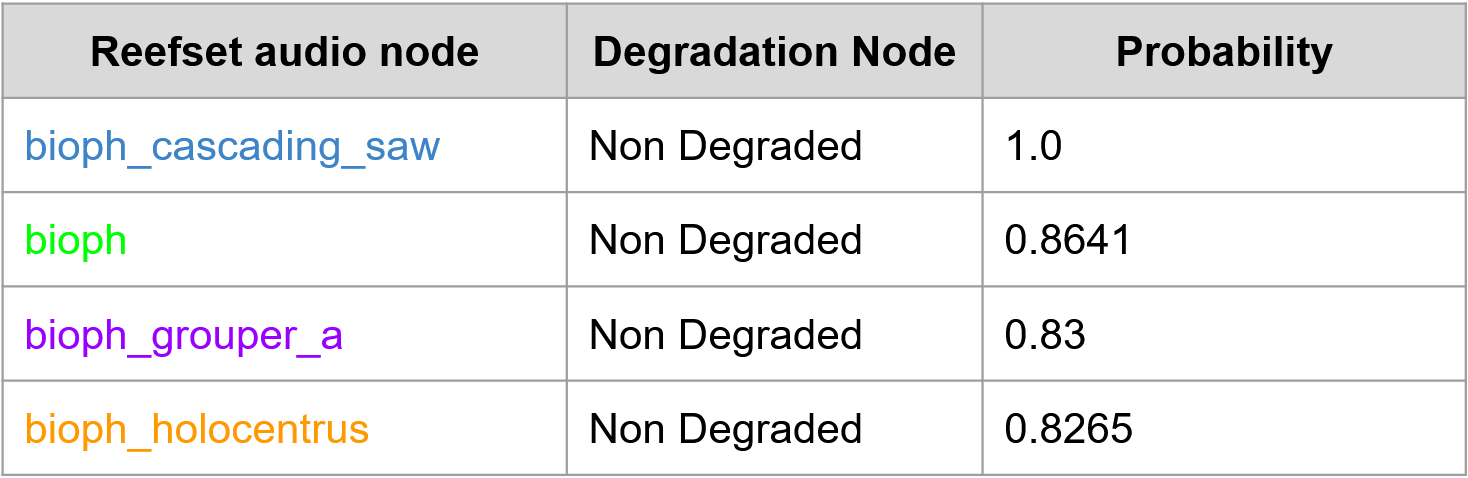
\includegraphics[height=1.0\textheight,width=1.0\textwidth,keepaspectratio]{images/knowledge_graph_table.png}
        \end{column}
        \begin{column}{0.3\textwidth}
            \centering
            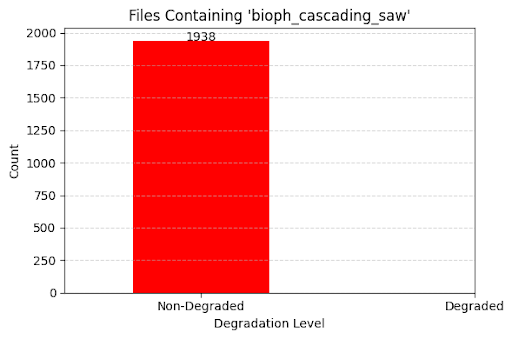
\includegraphics[height=1.0\textheight,width=1.0\textwidth,keepaspectratio]{images/knowledge_graph_results_1.png}
        \end{column}
    \end{columns}
    \hspace{1cm}
    \begin{columns}
        \begin{column}{0.33\textwidth}
            \centering
            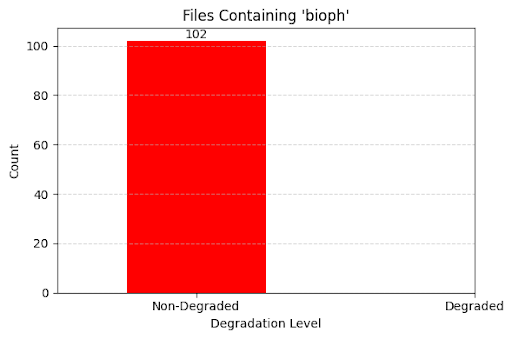
\includegraphics[height=1.0\textheight,width=1.0\textwidth,keepaspectratio]{images/knowledge_graph_results_2.png}
        \end{column}
        \begin{column}{0.33\textwidth}
            \centering
            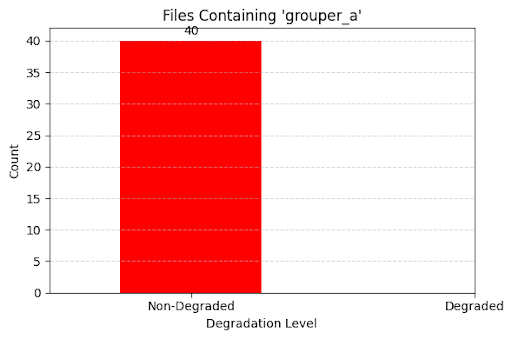
\includegraphics[height=1.0\textheight,width=1.0\textwidth,keepaspectratio]{images/knowledge_graph_results_3.png}
        \end{column}
        \begin{column}{0.33\textwidth}
            \centering
            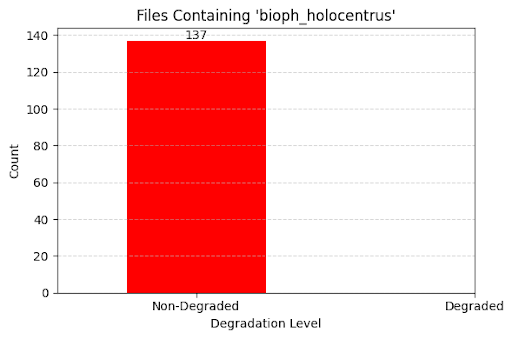
\includegraphics[height=1.0\textheight,width=1.0\textwidth,keepaspectratio]{images/knowledge_graph_results_4.png}
        \end{column}
    \end{columns}
\end{frame}

\begin{frame}{Knowledge Graphs - Future Work}
    \begin{itemize}
        \item Ensure future links are:
        \begin{itemize}
            \item Semantically cohesive (i.e. not predicting Dry Season $\rightarrow$ Degradation)
            \item Not a byproduct of a biased dataset
            \item Add more data (Costa Rica)
        \end{itemize}
        \item Ensure the graph is computational efficient
        \item Continue working on the binary classifier with Costa Rica data
        \item Work on knowledge graph visualization
    \end{itemize}
\end{frame}

\begin{frame}{Regression - Chi-Square Tests}
    \begin{figure}
        \centering
        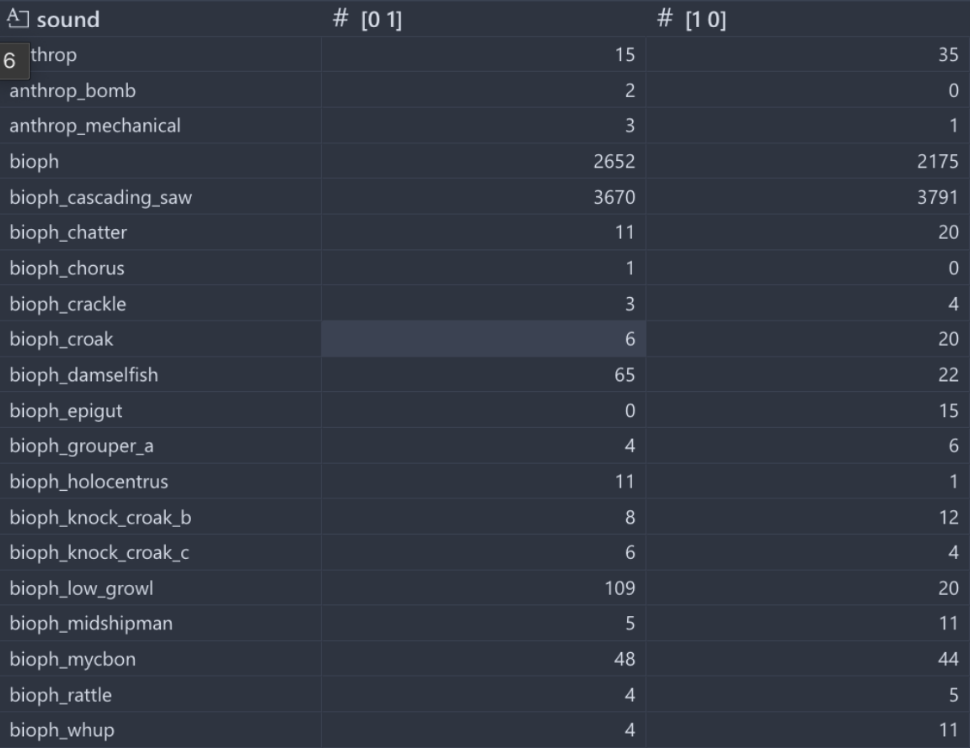
\includegraphics[height=0.8\textheight,width=0.8\textwidth,keepaspectratio]{images/reefset_classes.png}
        \caption{Occurrence of ReefSet classes in degraded and non-degraded reefs}
    \end{figure}
\end{frame}

\begin{frame}{Regression - Chi-Square Tests}
    \begin{figure}
        \centering
        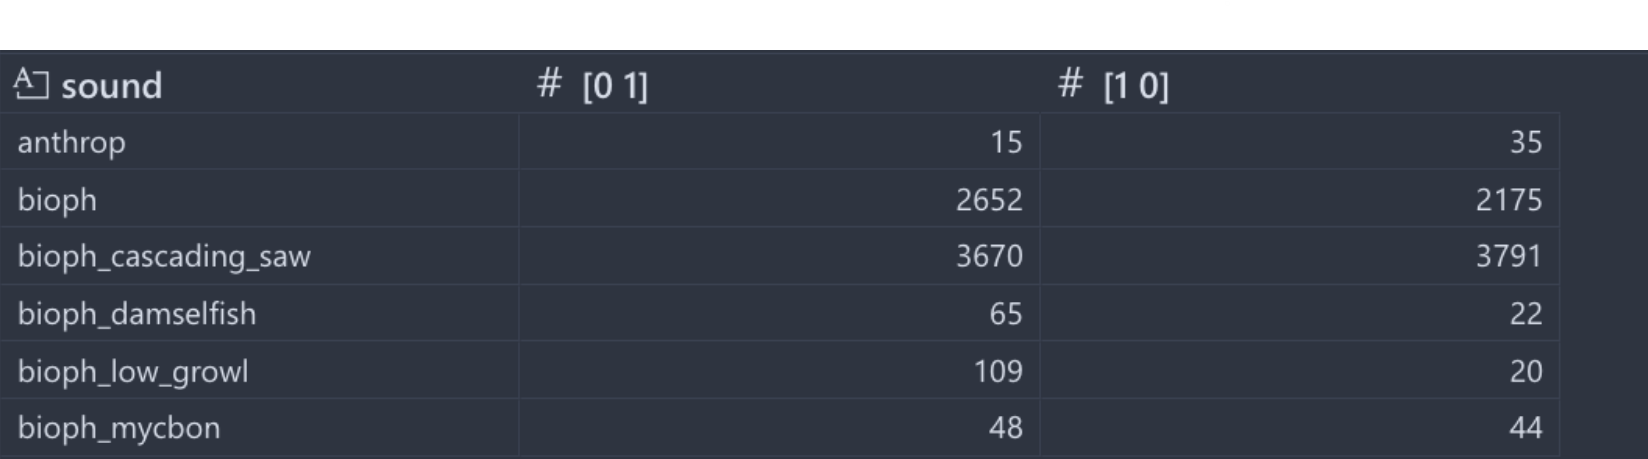
\includegraphics[height=0.8\textheight,width=0.8\textwidth,keepaspectratio]{images/chi_square_test.png}
        \caption{Classes with at least 30 occurrences in either degraded or non-degraded reefs}
    \end{figure}
    $\chi^2$: 523
    \newline
    P-value: $\sim$0
\end{frame}

\begin{frame}{Template Matching - Effectiveness}
    \begin{itemize}
        \item Able to find patterns but not the correct ones
            \begin{itemize}
                \item Domain shift, long/noisy xeno-canto templates cause issues
            \end{itemize}
    \end{itemize}
\end{frame}

\begin{frame}{Template Matching - Sound Separation}
    \begin{itemize}
        \item Exploring sound separation for better results
            \begin{itemize}
                \item Wisdom et al., 2020
            \end{itemize}
    \end{itemize}
    \begin{figure}
        \centering
        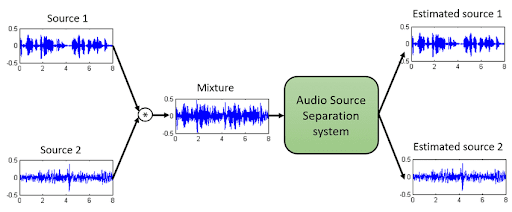
\includegraphics[height=0.7\textheight,width=0.7\textwidth,keepaspectratio]{images/sound_separation.png}
        \caption{Sound separation process (Duong, 2019)}
    \end{figure}
\end{frame}

\begin{frame}{Binary Classifier}
    \begin{columns}
        \begin{column}{0.5\textwidth}
            \begin{figure}
                \centering
                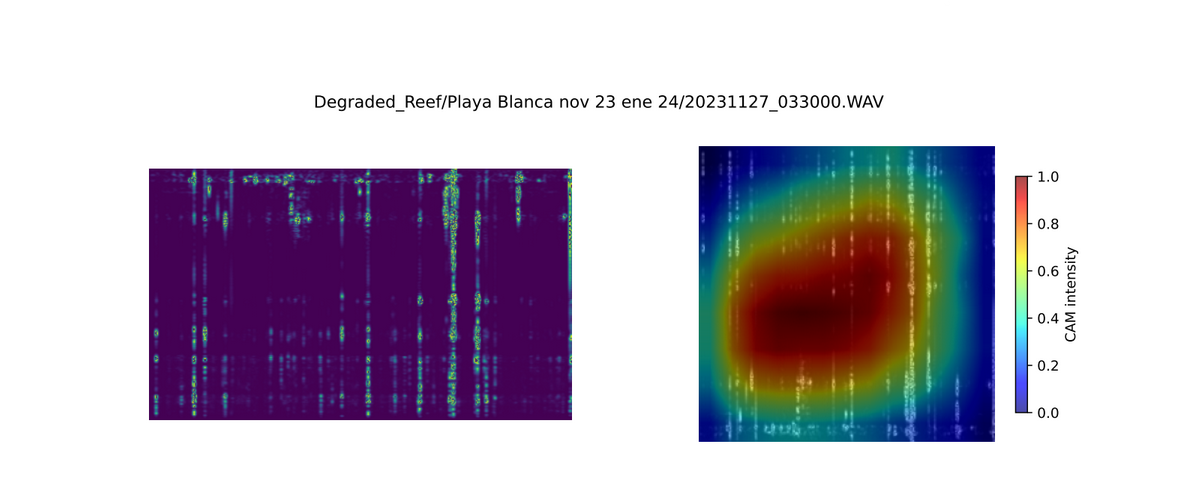
\includegraphics[height=0.75\textheight,width=0.75\textwidth,keepaspectratio]{images/degraded_gradcam.png}
                \caption{Degraded Grad-CAM}
            \end{figure}
        \end{column}
        \begin{column}{0.5\textwidth}
            \begin{figure}
                \centering
                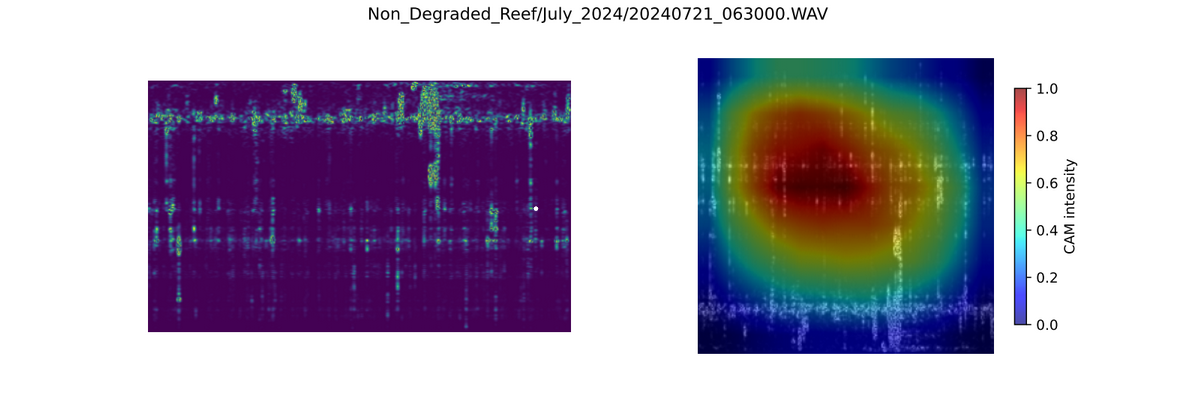
\includegraphics[height=0.75\textheight,width=0.75\textwidth,keepaspectratio]{images/non_degraded_gradcam.png}
                \caption{Non-degraded Grad-CAM}
            \end{figure}
        \end{column}
    \end{columns}
    \begin{figure}
        \centering
        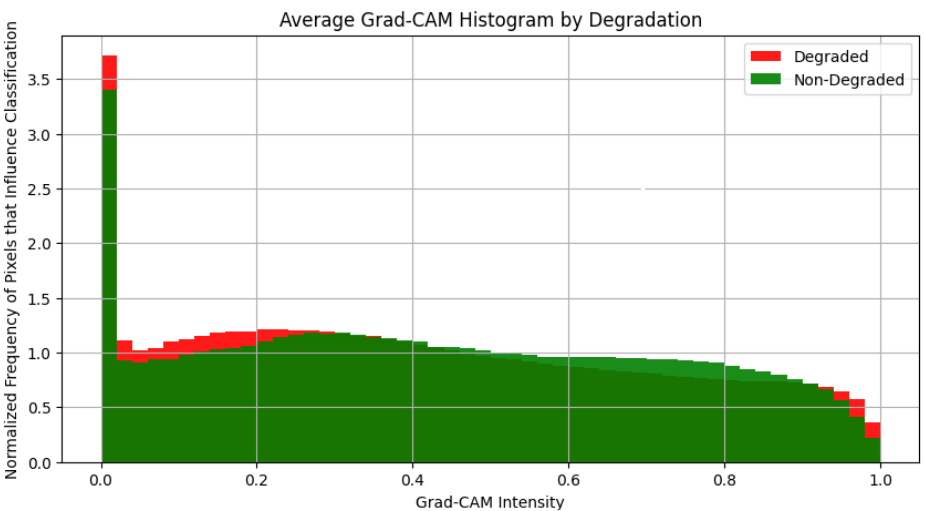
\includegraphics[height=0.5\textheight,width=0.5\textwidth,keepaspectratio]{images/gradcam_histogram.png}
        \caption{Grad-CAM histogram over 200 degraded and non-degraded samples}
    \end{figure}
\end{frame}

\begin{frame}{Binary Classifier}
    \begin{columns}
        \begin{column}{0.5\textwidth}
            \begin{figure}
                \centering
                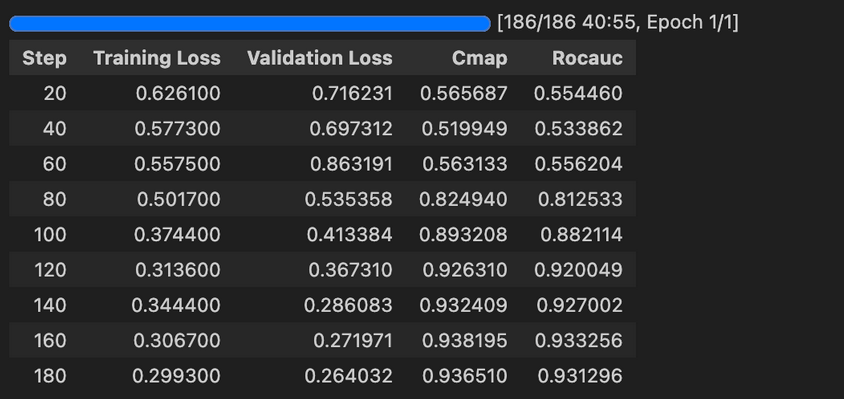
\includegraphics[height=1.0\textheight,width=1.0\textwidth,keepaspectratio]{images/binary_classifier_metrics_1.png}
                \caption{Binary classifier training metrics}
            \end{figure}
        \end{column}
        \begin{column}{0.5\textwidth}
            \begin{figure}
                \centering
                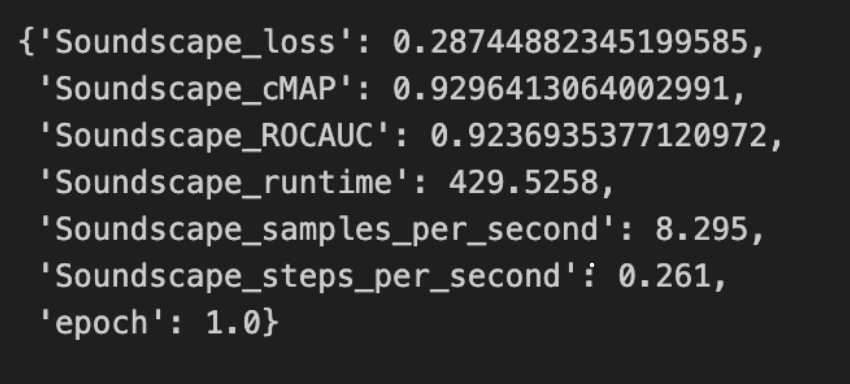
\includegraphics[height=1.0\textheight,width=1.0\textwidth,keepaspectratio]{images/binary_classifier_metrics_2.png}
                \caption{Final binary classifier metrics}
            \end{figure}
        \end{column}
    \end{columns}
\end{frame}

\begin{frame}{Site Separation}
    \begin{itemize}
        \item 
    \end{itemize}
\end{frame}

\begin{frame}{D3.JS Visualization}
    \begin{itemize}
        \item 
    \end{itemize}
\end{frame}

\begin{frame}{Autoencoders (Both Teams)}
    \begin{itemize}
        \item 
    \end{itemize}
    \begin{figure}
        \centering
        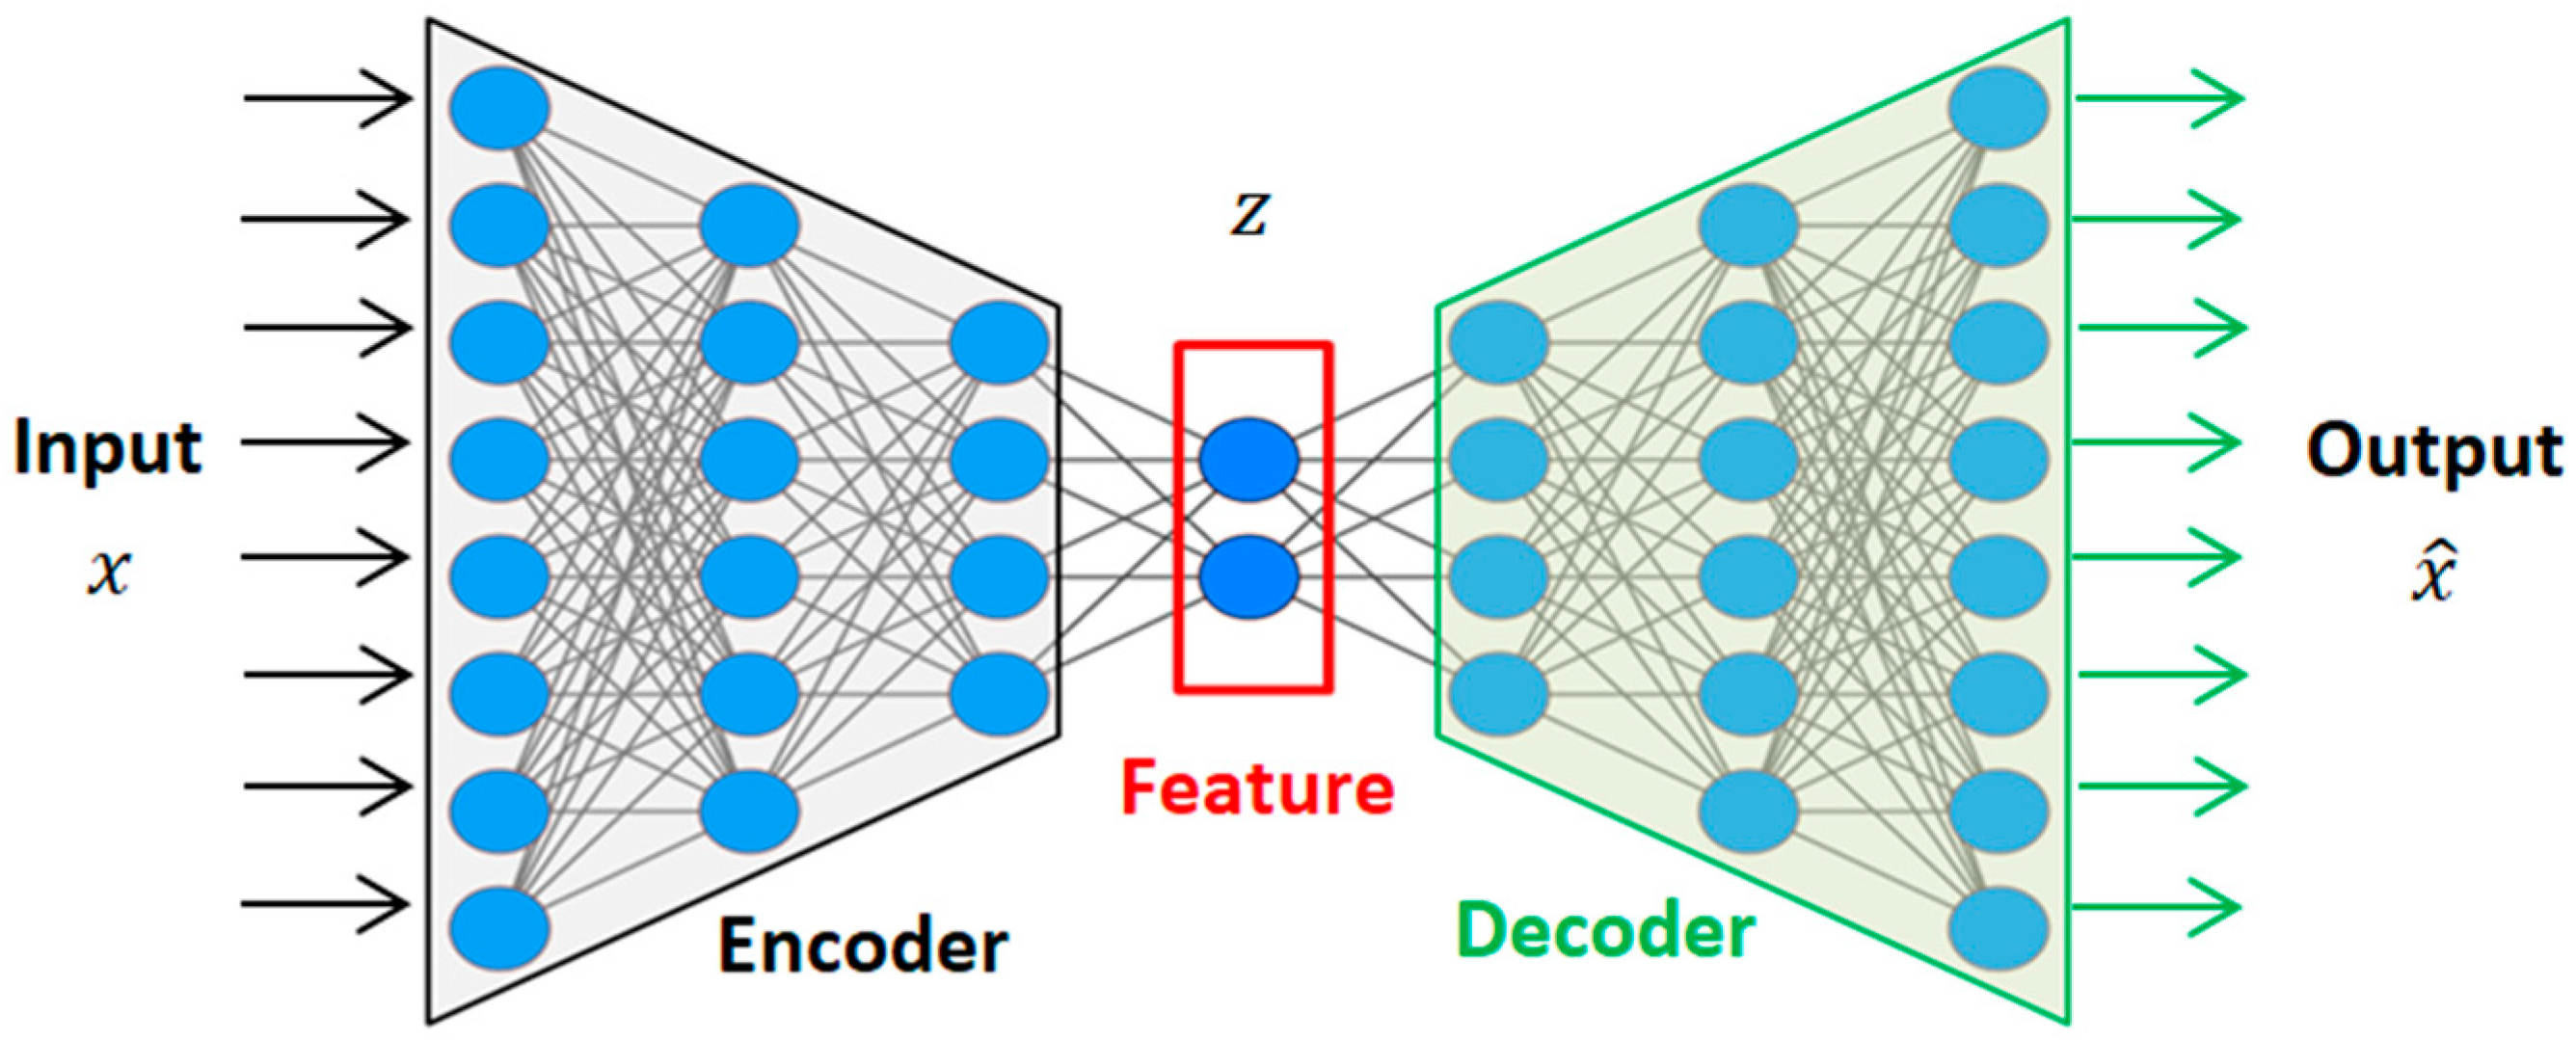
\includegraphics[height=0.7\textheight,width=0.7\textwidth,keepaspectratio]{images/autoencoder.png}
        \caption{Autoencoder architecture (Alaghbari et al., 2023)}
    \end{figure}
\end{frame}

\begin{frame}{Collar Team Agenda}
    \begin{itemize}
        \item 
    \end{itemize}
\end{frame}